\documentclass{article} % For LaTeX2e
\usepackage{nips15submit_e,times}
\usepackage{hyperref}
\usepackage{url}
%\documentstyle[nips14submit_09,times,art10]{article} % For LaTeX 2.09

\usepackage{hyperref}
\usepackage{url}
\usepackage[utf8x]{inputenc}
\usepackage[english]{babel}
\usepackage{natbib}
\usepackage{nicefrac}
\usepackage{algorithm}
\usepackage{algorithmic}
\usepackage{amsfonts}
\usepackage{graphics}
\usepackage{graphicx}
\usepackage{tikz}
\usetikzlibrary{bayesnet}
\tikzstyle{connect}=[-latex]
\tikzstyle{allconnected}=[line width=0.1cm]

%\usepackage{verbatim}
%\usepackage[active,tightpage]{preview}
%\PreviewEnvironment{tikzpicture}
%\usepackage{savetrees}

\def\bbbr{{\rm I\!R}}
\newcommand{\vp}{\vec{\phi}}
\newcommand{\vmu}{\vec{\mu}}
\newcommand{\vf}{\vec{f}}

\newcommand{\vm}{\vec{m}}
\newcommand{\vx}{\vec{x}}
\newcommand{\vr}{\vec{r}}
\newcommand{\vy}{\vec{y}}
\newcommand{\vz}{\vec{z}}
\newcommand{\vY}{\vec{Y}}
\newcommand{\vX}{\vec{X}}
\newcommand{\bx}{\textbf{x}}
\newcommand{\bz}{\textbf{z}}
\newcommand{\bw}{\textbf{w}}
\newcommand{\by}{\textbf{y}}
\newcommand{\bL}{\textbf{L}}
\newcommand{\bI}{\textbf{I}}
\newcommand{\vk}{\vec{k}}
\newcommand{\vL}{\vec{\Lambda}}
\newcommand{\xmin}{x_{\min}}
\newcommand{\pmin}{p_{\min}}
\newcommand{\fmin}{f_{\min}}
\newcommand{\hpmin}{\hat{p}_{\min}}
\newcommand{\hqmin}{\hat{q}_{\min}}
\newcommand{\pfmin}{p_{f_{\min}}}
\renewcommand{\vec}{\boldsymbol}
\newcommand{\fun}[1]{\mathsf{#1}}
\renewcommand{\O}{\mathcal{O}}
\newcommand{\GP}{\mathcal{GP}}
\newcommand{\N}{\mathcal{N}}
\newcommand{\Id}{\vec{I}}
\newcommand{\II}{\mathbb{I}}
\newcommand{\IR}{\mathbb{R}}

\newcommand{\tr}{\operatorname{tr}}
\newcommand{\argmin}{\operatorname*{arg\: min}}
\newcommand{\argmax}{\operatorname*{arg\: max}}
\newcommand{\chol}{\operatorname{\mathsf{C}}}

\newcommand{\data}{\mathcal{D}}
\newcommand{\reals}{\mathbb{R}}
\newcommand{\sX}{\mathcal{X}}
\newcommand{\xst}{x_{\ast}}
\newcommand{\yst}{y_{\ast}}

\usepackage{xspace}
\newcommand{\acr}[1]{\textsc{#1}\xspace}
\newcommand{\gp}{\acr{gp}}
\newcommand{\dpp}{\acr{dpp}}
\newcommand{\us}{\acr{glasses}}

\newtheorem{theorem}{Theorem}
\newtheorem{lemma}{Lemma}
\newtheorem{corollary}{Corollary}
\newtheorem{proposition}{Proposition}
\newtheorem{definition}{Definition}
\newtheorem{proof}{Proof}
\newtheorem{conjecture}{Conjecture}



\graphicspath{{./},{./figs/}}




\title{
    GLASSES: Relieving The Myopia Of Bayesian Optimisation
}
    
 
\author{
David S.~Hippocampus\thanks{ Use footnote for providing further information about author (webpage, alternative address)---\emph{not} for acknowledging funding agencies.} \\
Department of Computer Science\\
Cranberry-Lemon University\\
Pittsburgh, PA 15213 \\
\texttt{hippo@cs.cranberry-lemon.edu} \\
\And
Coauthor \\
Affiliation \\
Address \\
\texttt{email} \\
}

\newcommand{\fix}{\marginpar{FIX}}
\newcommand{\new}{\marginpar{NEW}}

%\nipsfinalcopy % Uncomment for camera-ready version

    
\begin{document}

\maketitle

\begin{abstract}
    We present \us: Global optimisation with Look-Ahead through Stochastic Simulation and Expected-loss Search. 
    The vast majority of global optimisation approaches in use are myopic, in only considering the impact of the next function value; the remaining approaches are able to consider only a handful of future evaluations. 
    Our novel algorithm, \us, permits the consideration of dozens of evaluations into the future. 
    We show that the far-horizon planning thus enabled leads to substantive performance gains in empirical tests. 
\end{abstract}

\section{Introduction} % (fold)
\label{sec:introduction}

Almost all global optimisation techniques are myopic, in considering no more than a single step into the future. 
We define the multi-step lookahead problem as the global optimisation of an function by considering the significance of the next function evaluation on function evaluations (steps) further into the future. 
It is clear that a solution to the problem would offer performance gains.
For example, consider the case in which we have a budget of two evaluations with which to optimise a function $f(x)$ over the domain $\sX = [0, 1] \subset \reals$. 
If we are strictly myopic, our first evaluation will likely be at 
$x=\nicefrac{1}{2}$, and our second then at only one of $x=\nicefrac{1}{4}$ and $x=\nicefrac{3}{4}$. 
This myopic strategy thereby ignores half of the domain $\sX$, regardless of the second choice. 
If we adopt a two-step lookahead approach, we will select function evaluations that will be more evenly distributed across the domain by the time the budget is exhausted, and will hence be more informative about $f$ and its optimum.

There is a limited literature on the multi-step lookahead problem.
\cite{osborne_gaussian_2009} perform multi-step lookahead by optimising future evaluation locations, and sampling over future function values. 
This approach scales poorly with the number of future evaluations considered, and the authors present results for no more than two-step lookahead.
\cite{Marchant*Ramos*Sanner*2014} reframe the multi-step lookahead problem as a partially observed Markov decision process, and adopt a Monte Carlo tree search approach in solving it. 
Again, the scaling of the approach permits the authors to consider no more than six steps into the future. 

There is a clear link between the multi-step lookahead problem and that considered in the literature as \emph{batch} Bayesian optimisation. 
The two problems are distinct but related: the multi-step lookahead problem requires the challenging marginalisation over unknown future evaluation \emph{locations}, in addition to the unknown future evaluation \emph{values} also marginalised by batch approaches. 
Similarly to the state-of-the-art in multi-step lookahead, the batch literature provides only poor scaling with the number of evaluations.
\cite{Ginsbourger2009} present results for no more than six simultaneous function evaluations.\cite{Azimi2012,Azimi2011} use the surrogate model for $f$ to generate `fake' observations and avoid the marginalization step. This produce a large acumulation of errors that does not allow the use these techniques for the collection of large batches.


We propose an algorithm, \us, that provides scaling superior to existing alternatives.

% section introduction (end)

\begin{figure}
\centering
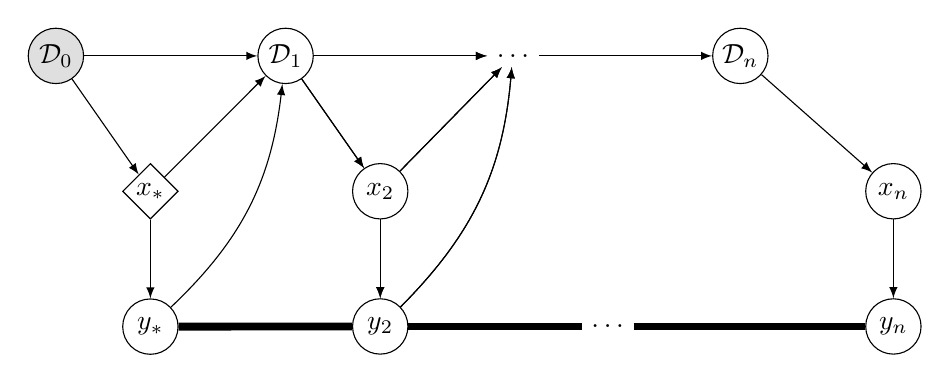
\begin{tikzpicture}

    % first row
    \node[obs] (D0) {$\data_0$};
    \node[latent, right=of D0, xshift=1.2cm] (D1) {$\data_1$};
    \node[draw=none, right=of D1, xshift=1.2cm] (Ddots) {$\ldots$};
    \node[latent, right=of Ddots, xshift=1.2cm] (Dn) {$\data_n$};

    % second row
    \node[det, below=of D0, xshift=1.2cm] (xst) {$\xst$};
    \node[latent, right=of xst, xshift=1.2cm] (x2) {$x_2$};
    \node[latent, right=of x2, xshift=4.8cm] (xn) {$x_n$};

    % third row
    \node[latent, below=of xst] (yst) {$\yst$};
    \node[latent, below=of x2] (y2) {$y_2$};
    \node[draw=none, right=of y2, xshift=1.2cm] (ydots) {$\ldots$};
    \node[latent, below=of xn] (yn) {$y_n$};

    % Connect the nodes
    \path 
        (D0) edge [connect] (D1)
        (D0) edge [connect] (xst)
        (xst) edge [connect] (yst)
        (xst) edge [connect] (D1)
        (yst) edge [connect, bend right=20] (D1)
        (yst) edge [allconnected] (y2)

        (D1) edge [connect] (Ddots)
        (D1) edge [connect] (x2)
        (x2) edge [connect] (y2)
        (x2) edge [connect] (Ddots)
        (y2) edge [connect, bend right=20] (Ddots)
        (y2) edge [allconnected] (ydots)

        (D1) edge [connect] (Ddots)
        (D1) edge [connect] (x2)
        (x2) edge [connect] (y2)
        (x2) edge [connect] (Ddots)
        (y2) edge [connect, bend right=20] (Ddots)
        (ydots) edge [allconnected] (yn)

        (Ddots) edge [connect] (Dn)
        (Dn) edge [connect] (xn)
        (xn) edge [connect] (yn)        
        ;
\end{tikzpicture}
\caption{
    A Bayesian network describing the $n$-step lookahead problem. The shaded node ($\data_0$) is known, and the diamond node ($\xst$) is the current decision variable. All $y$ nodes are correlated with one another under the \gp model.
}
\label{fig:bayes_net}
\end{figure}


\section{Conditional DPPs for step ahead locations}

To approximate $\Lambda_n(\bx_*)$ we compute  $E_{p(\by)} [\min (\by,\eta)]$ where $\by=\{y_1,\dots,y_n\}$ with $p(\by) \sim \N(\by; \mu, \Sigma)$ is the multivariate random vector that we obtain after evaluation the predictive distribution of the \gp at locations $\bx_*,\bx_2,\dots,\bx_n$. Point $\bx_*$ is fixed (is the point where we evaluate $\Lambda_n$) and we consider $\bx_2,\dots,\bx_n$ to be a sample of the conditional k-\dpp (for $k=n$) on $\bx_*$ with kernel $L$ (in principle, the one from the \gp).
 
Let $\bL$ be the kernel matrix corresponding to the evaluation of $L$ on a finite set $\Omega$ of potential points (pre-uniformly sampled in the domain of interest, for instance).  The distribution obtained by conditioning on having observed $\bx_* \in \Omega$ can be obtained as follows. Let $B \subset \Omega$ a non intersecting set with $\bx_*$. We have that
\begin{eqnarray}
p_L(\bx_* \cup B | \bx_* \subseteq Z ) = \frac{p_L(Z = \bx_* \cup B ) }{p(\bx_* \subseteq Z)} = \frac{\det(\bL_{\bx_* \cup B})}{\det(\bL - \bI_{\bar{\bx}_*} ) }
\end{eqnarray}
where $\bI_{\bar{\bx}_*}$ is the matrix with ones in the diagonal entries indexed by elements of $\Omega - \bx_*$ and zeros elsewhere.  This conditional distribution is again a \dpp over subsets of $\Omega-\bx_*$ \citep{Borodin*Rains*2005} with kernel 
$$\bL^{\bx_*} = \left( [   (\bL + \bI_{\bar{\bx}_*})^{-1}]_{\bar{\bx}_*} \right)^{-1}.$$
$[\cdot ]_{\bar{\bx}_*}$ represents the restriction of the matrix to all rows and columns not indexed by $\bx_*$. The previous inverses exist if and only if the probability of $\bx_*$ appearing is nonzero, as is the case in our context. A second marginalization is later needed to generate samples of size k.  Figure \ref{fig1} shows an example of samples from a k-\dpp and a conditional k-\dpp with the same kernel.
 
\begin{figure}[ht]
    \centering
  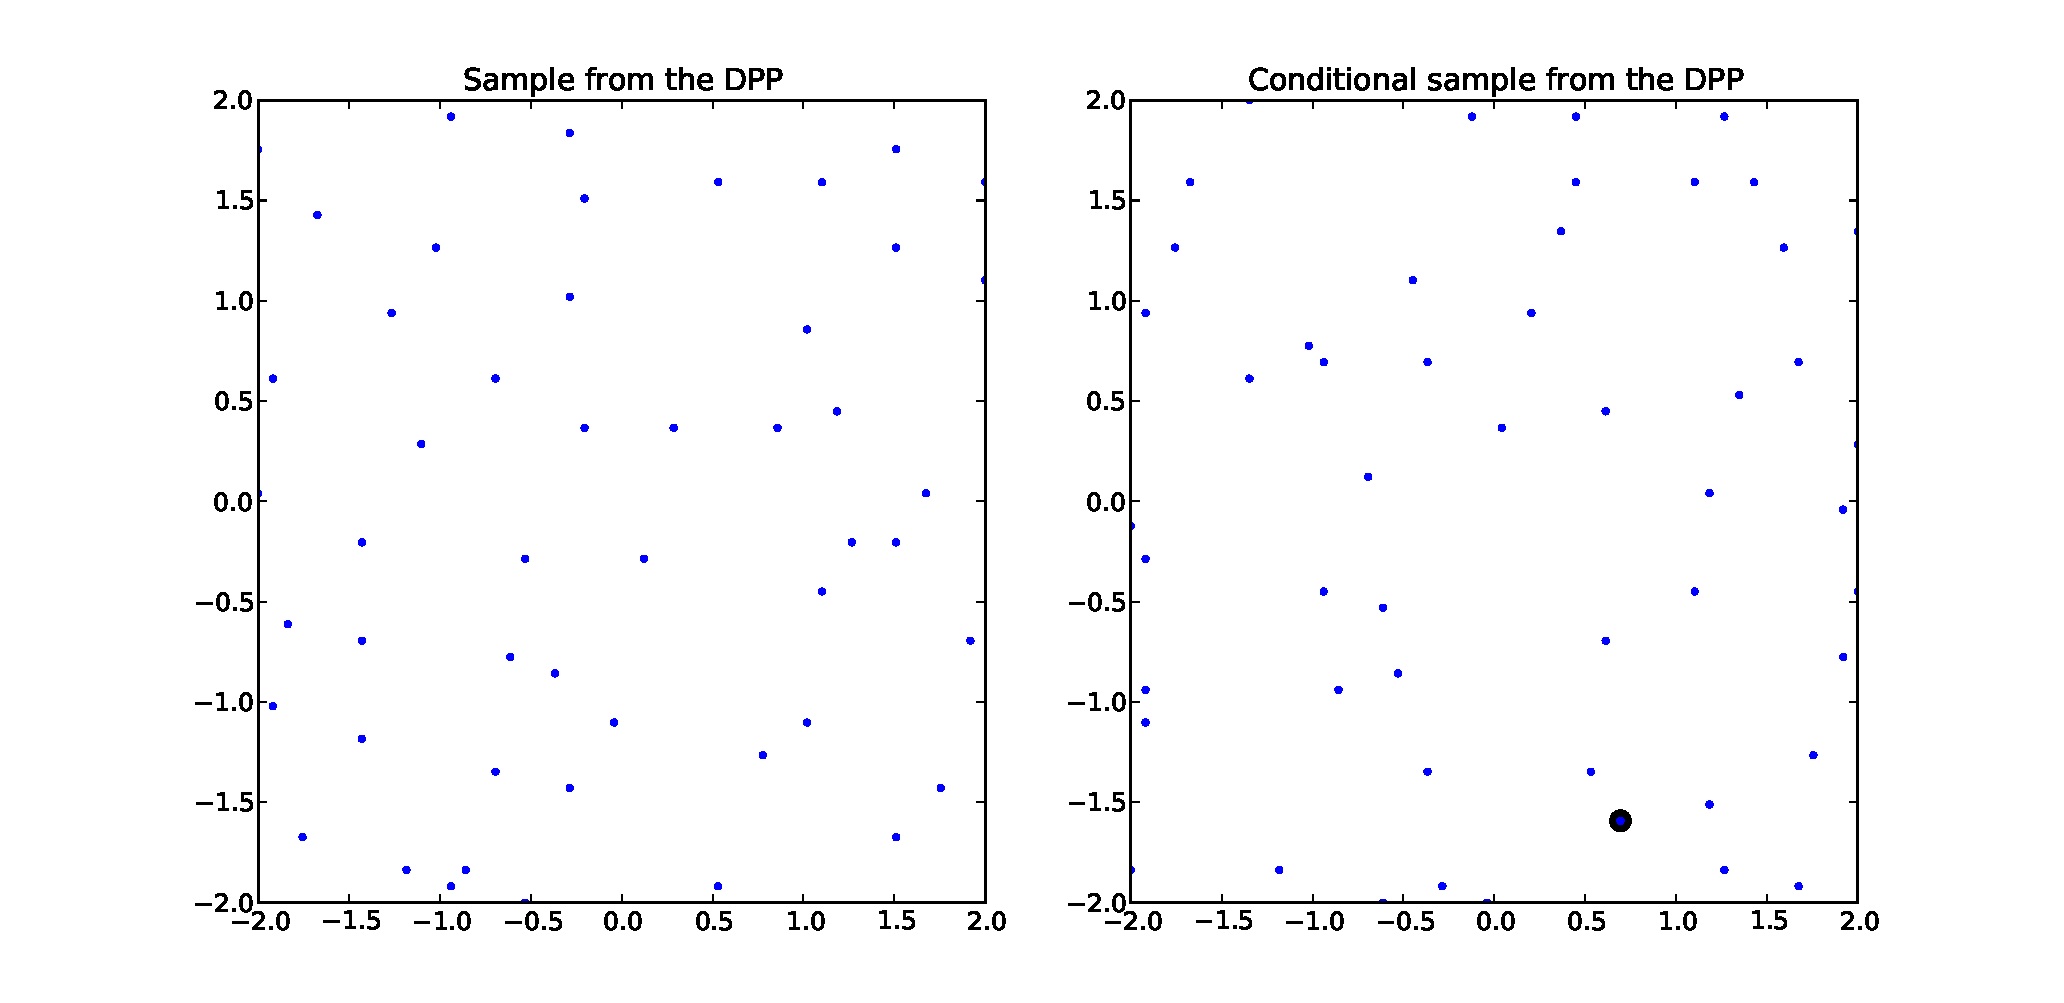
\includegraphics[width=.9\textwidth]{conditional_dpp.pdf}
\caption{Left: sample from a k-\dpp (k=50) for a SE kernel with length-scale 0.5. Right: sample from a k-\dpp (k=50) conditional to $x_1$ (black dot) being in the selected set. }
    \label{fig1}
\end{figure}

\newpage
\section{Computation of the Expected loss}
Our goal is to compute $E_{p(\by)} [\min (\by,\eta)]$ for $\by=\{y_1,\dots,y_n\}$ and $p_0(\by) \sim \N(\by; \mu, \Sigma)$. This  approximates the n-steps ahead expected loss $\Lambda_n(\bx_*)$. The goal of this section is to write  $E_{p(\by)} [\min (\by,\eta)]$ in a way that it is suitable to be computed by Expectation Propagation. Next proposition will do the work (I think).

\begin{proposition}

\begin{equation}\label{eq:expected_loss}
E_{p(\by)} [\min (\by,\eta)] =  \sum_{j=1}^n  \int_{\IR^n} y_j \prod_{i=1}^n t_{j,i}(\by) \N(\by; \mu, \Sigma) d \by + \eta\int_{\IR^n} \prod_{i=1}^nh_i(\by) \N(\by; \mu, \Sigma) d\by
\end{equation}
where  $h_i(\by) = \mathbb{I}\{y_i>\eta\}$ and
$$t_{j,i}(\by)= \left\{ \begin{array}{lcl}
\mathbb{I}\{y_j \leq\eta\} & \mbox{ if } $ i=j$ \\
  \\
 \mathbb{I}\{ 0 \leq y_i-y_j \} &   \mbox{otherwise.} 
\end{array}
\right.$$

\end{proposition}



\begin{proof}
Denote by 
\begin{eqnarray}\nonumber
E_{p(\by)} [\min (\by,\eta)] & = & \int_{\IR^n} \min (\by,\eta)  \N(\by; \mu, \Sigma) d\by\\ \nonumber
& = & \int_{\IR^n - (\eta,\infty)^n } \min (\by)  \N(\by; \mu, \Sigma) d\by + \int_{(\eta,\infty)^n} \eta  \N(\by; \mu, \Sigma) d\by  \nonumber
\end{eqnarray}

The first term can be written as follows:

\begin{equation}
 \int_{\IR^n - (\eta,\infty)^n } \min (\by)  \N(\by; \mu, \Sigma) d\by  =    \sum_{j=1}^n \int_{P_j} y_j \N(\by; \mu, \Sigma) d \by \nonumber
\end{equation}\nonumber

where $P_j := \{ \by \in\IR^n - (\eta,\infty)^n  : y_j \leq y_i,\,\, \forall i \neq j \}$. We can do this because the regions $P_j$ are disjoint and it holds that $\cup_{j=1}^{n}P_j = \IR^n - (\eta,\infty)^n $.  Also, note that the $\min(\by)$ can be replaced within the integrals since within each $P_j$ it holds that $\min(\by) = y_j$. Rewriting the integral in terms of indicator functions we have that
\begin{eqnarray}\label{eq:term1}
 \sum_{j=1}^n \int_{P_j} y_j \N(\by; \mu, \Sigma) d \by   =  \sum_{j=1}^n  \int_{\IR^n} y_j \prod_{i=1}^n t_{j,i}(\by) \N(\by; \mu, \Sigma) d \by 
\end{eqnarray}

where $t_{j,i}(y) =\mathbb{I}\{y_i \leq\eta\}$ if $j=i$ and $t_{j,i}(y) =\mathbb{I}\{y_j \leq y_i \}$ otherwise.

The second term can be written as
\begin{equation}\label{eq:term2}
 \int_{(\eta,\infty)^n } \eta  \N(\by; \mu, \Sigma) d\by = \eta\int_{\IR^n} \prod_{i=1}^nh_i(\by) \N(\by; \mu, \Sigma) d\by
\end{equation}
where $h_i(\by) = \mathbb{I}\{y_i>\eta\}$.  Merge (\ref{eq:term1}) and (\ref{eq:term2}) to conclude the proof.
 
\end{proof}

All the elements in (\ref{eq:expected_loss}) can be rewritten in a way that can be computed using EP but the work in \cite{Cunningham*Hennig*Lacoste-Julien_2011}. 

\begin{itemize}
\item The second term is a Gaussian probability on unbounded polyhedron in which the limits are aligned with the axis.  
\item The first term requires some more processing but it is still computable under the assumptions in \cite{Cunningham*Hennig*Lacoste-Julien_2011}. Let $\bw_j$ the $jth$ canonical vector. Then we have that
\begin{eqnarray}
\int_{\IR^n} y_j \prod_{i=1}^n t_{j,i}(\by) \N(\by; \mu, \Sigma) d \by & = & \bw^T  \int_{\IR^n} \by \prod_{i=1}^n t_{j,i}(\by) \N(\by; \mu, \Sigma) d \by \\
& = & \bw^T E[\by] z_j
\end{eqnarray}
where the expectation is calculated over the normalized distribution over $P_j$, the one EP approximates with $q(\by)$, and for $z_j$ being the normalizing constant 
  $$z_j= \int_{\IR^n} \prod_{i=1}^n t_{j,i}(\by) \N(\by; \mu, \Sigma) d \by$$  
Because EP does moments matching, both the normalizing constant and the expectation are available.
\end{itemize}



\begin{algorithm}[t!]
   \caption{Decission process of the \us algorithm.}
   \label{alg:glasses}
\begin{algorithmic}
   \STATE {\bfseries Input:} dataset $\mathcal{D}_{0} = \{(\textbf{x}_0, y_0)\}$, number of remaining evaluations ($n$), representer points ($r$) and \dpp replicates (s).
\STATE
   \STATE Fit a \gp with kernel $k$ to $\mathcal{D}_{0}$.
   \STATE Select $\bx_{1*},\dots,\bx_{r*}$ representer points of the loss.
   \FOR{$j=1$ {\bfseries to} $r$ }
   \STATE Take $s$ samples from a conditional n-\dpp of kernel $k$ given $\bx_{j*}$.
   \STATE Approximate the expected loss at $\bx_j^*$ for the $s$ samples computing $E [\min (\by,\eta)]$.
  \STATE Average the expected loss for the $s$ samples and obtain $\tilde{\Lambda}_n(\bx_j^*)$.
   \ENDFOR
\STATE Approximate $\Lambda_n(\bx_*)$ fitting a $\gp_2$  to $\{(\bx_{j*}, \tilde{\Lambda}_n(\bx_{j*})\}_{j=1}^r$ with posterior mean $\mu_2$.
   \STATE \textbf{Returns}: New location at $\arg \min_{x \in \mathcal{X}} \left\{\mu_2(\bx)\right\}$.  
\end{algorithmic}
\end{algorithm}



\bibliographystyle{plain}
\bibliography{bib_glasses}

\end{document}
